\chapter{Notes}\label{chap:Notes}

\section{Complexity of matrix multiply}\label{sec:Complexity of matrix multiply}

Assume $\mathbf{A}$ is $m\times n$ and $\mathbf{B}$ is $n\times p$.
The naive algorithm takes $O\left(mnp\right)$ time.


\section{Representation of matrix}\label{sec:Representation of matrix}

Row major, col major, stride


\paragraph{How to calculate dimension of convolutional layer} % (fold)

\[ \left\lfloor \frac{n_h - k_h + p_h + s_h}{s_h} \right\rfloor \times \left\lfloor \frac{n_w - k_w + p_w + s_w}{s_w} \right\rfloor \]
In which  \(n_h\)  means height of input, \(k_h\) means height of filter, \(p_h\) means padding of height, \(s_h\) means stride of height. So as \(n_w\), \(k_w\), \(p_w\), \(s_w\).


\section{Training Tricks}\label{sec:Training skills}


\paragraph{Batch normalization}

\[ \textrm{BN}\left(\bm{x}\right)  = \gamma  \odot \frac{\bm{x} - \hat{\bm \mu}_\mathcal{B}}{\hat{\bm \sigma}_\mathcal{B}} + \beta
\]

Batch normalization is a technique that drastically reduces this problem.
The solution is surprisingly simple.
During training, a batch normalization layer calculates the mean and standard deviation of each of its input channels across the batch and normalizes by subtracting the mean and dividing by the standard deviation.
There are then two learned parameters for each channel, the scale (gamma) and shift (beta)~\cref{fig:batch_normalization}.
The output is simply the normalized input, scaled by gamma and shifted by beta~\cite{foster2022generative}.


When it comes to prediction, we may only want to predict a single observation, so there is no batch over which to calculate the mean and standard deviation.
To get around this problem, during training a batch normalization layer also calculates the moving average of the mean and standard deviation of each channel and stores this value as part of the layer to use at test time~\cite{foster2022generative}.

How many parameters are contained within a batch normalization layer? For every channel in the preceding layer, two weights need to be learned: the scale (gamma) and shift (beta).
These are the trainable parameters.
The moving average and standard deviation also need to be calculated for each channel, but since they are derived from the data passing through the layer rather than trained through backpropagation, they are called nontrainable parameters.
In total, this gives four parameters for each channel in the preceding layer, where two are trainable and two are nontrainable~\cite{foster2022generative}.

\begin{figure}
	\begin{center}
		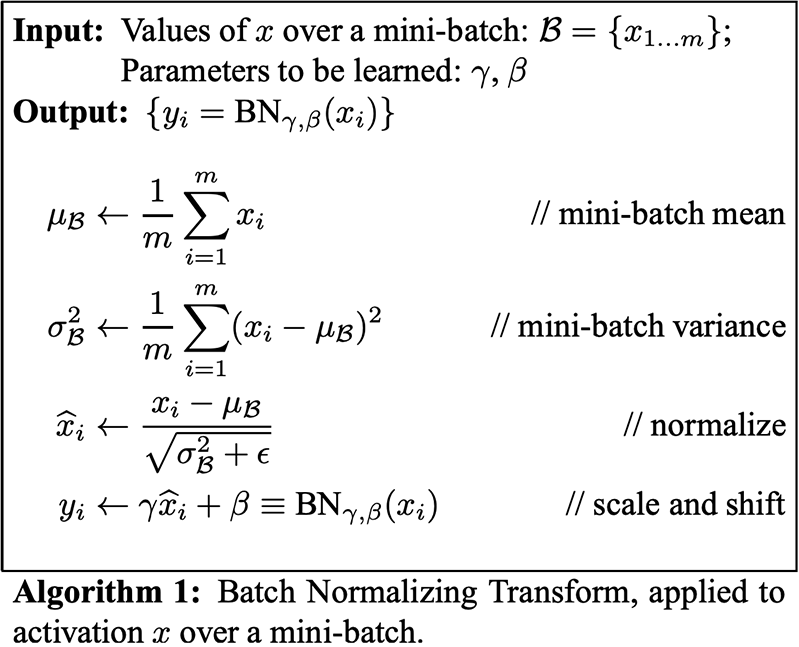
\includegraphics[width=0.95\textwidth]{figures/batch_normlization_page_76}
	\end{center}
	\caption{Batch Normalization}\label{fig:batch_normalization}
\end{figure}


\paragraph{Transposed Convolution}


\cite{zhang2023dive}




% chapter Notes (end)
